\documentclass[12pt]{article}
\usepackage{amsfonts,amsthm,amsmath,amssymb,mathtools}
\usepackage{mathrsfs}
\usepackage{enumitem}
\usepackage{tikz-cd}
\usepackage{geometry}
\usepackage{mlmodern}
\usepackage{graphicx}

\geometry{letterpaper, portrait, margin=1in}

\setcounter{section}{0}

\renewcommand{\thesection}{\S\arabic{section}}
\renewcommand{\thesubsection}{\arabic{section}}
\DeclareMathOperator{\im}{im}

\newtheorem{thm}{Theorem}
\newenvironment{theorem}[1]{
	\renewcommand{\thethm}{#1}
	\begin{thm}
		}{\end{thm}}

\newtheorem{lma}{Lemma}
\newenvironment{lemma}[1]{
	\renewcommand{\thelma}{#1}
	\begin{lma}
		}{\end{lma}}

\theoremstyle{definition}
\newtheorem{ex}{Assignment}
\newenvironment{exercise}[1]{
	\renewcommand{\theex}{#1}
	\begin{ex}
		}{\end{ex}}

\title{MTH 732 Topology - Homework 2}
\author{Connor Mooneyhan}
\date{January 29, 2026}

\begin{document}

\maketitle

\begin{ex}
	Show that if $A$ is a strong deformation retract of $X$, then the inclusion $i : A \hookrightarrow X$ induces an isomorphism of fundamental groups.
\end{ex}
\begin{proof}
	We already know that $i_*$ is a group homomorphism, so we just need to show that it is bijective.
	To show that it is surjective, let $F: X \times [0, 1] \to X$ be a deformation retraction of $X$ onto $A$, let $x_0 \in A$, and let $[\gamma]_X \in \pi_1(X, x_0)$.
	Now define $G : [0, 1]^2 \to X$ by $G_t(a) \mapsto F_t(\gamma(a))$.
	Then $G_0 = \gamma$, $\im G_1 \subset A$, and $G_t(0) = G_t(1) = x_0$ since $x_0 \in A$ and $F_t|_A = \mathrm{id}_A$.
	Thus $G$ is a path homotopy from $\gamma$ to $G_1$, so $[\gamma]_X = [G_1]_X = i([G_1]_A)$, where $[G_1]_A \in \pi_1(A, x_0)$.

	For injectivity, let $\alpha, \beta \in \pi_1(A, x_0)$ such that $i_*([\alpha]) = i_*([\beta])$.
	Then there exists a path homotopy $H : [0, 1]^2 \to X$ such that $H_0 = \alpha$ and $H_1 = \beta$.
	We can then define $K = F_1 \circ H : [0, 1]^2 \to A$, which is continuous since both $H$ and the retraction $F_1$ are continuous.
	Moreover, $K_t(0) = H_t(0) = \alpha(0) = \beta(0)$ and $K_t(1) = H_t(1) = \alpha(1) = \beta(1)$ since $F_1$ is constant on $A$ and the endpoint $x_0$ is in a.
	Finally, $K_0 = \alpha$ and $K_1 = \beta$, again since $F_1$ is constant on $A$.
	Thus, $K$ is a path homotopy from $\alpha$ to $\beta$ in A, so $[\alpha]_A = [\beta]_A$ as desired.
\end{proof}

\begin{ex}
	Let $p : E \to B$ be a covering map.
	Show that if $E$ is path-connected and $B$ is simply-connected\footnote{This means $B$ is path-connected and has trivial fundamental group.}, then $p$ is a homeomorphism.
\end{ex}
\begin{proof}
	We know that $p$ is surjective by definition, so we show that $p$ is injective.
	Let $e_0, e_1 \in E$ such that $p(e_0) = p(e_1) = b_0$.
	Then there exists a path $\beta$ connecting $e_0$ to $e_1$ since $E$ is path-connected.
	Let $\alpha = p(\beta)$.
	Then $[\alpha] \in \pi_1(B, b_0)$, and since $B$ is simply connected, we have a path homotopy $H : [0, 1]^2 \to B$ from $\alpha$ to the constant path $f_{b_0} : [0, 1] \to \lbrace b_0 \rbrace$.
	This lifts to a path homotopy $\widetilde{H}$ from $\beta$ to some path $\gamma : [0, 1] \to p^{-1}(b_0)$ with $\gamma(0) = e_0$.
	Since $p^{-1}(b_0)$ is a discrete set, we must have that $\gamma$ is actually constant, and thus is in particular the constant path at $e_0$.
	Since $\widetilde{H}$ is a \textit{path} homotopy, however, it must fix endpoints, and thus $e_0 = e_1$.
	Therefore $p$ is injective.

	Now we need to show that $p^{-1}$ is continuous.
	Let $x \in B$, let $V$ be a neighborhood of $p^{-1}(x)$, and let $U$ be an evenly covered neighborhood of $x$.
	The fact that $p$ is a covering map tells us that $p|_{p^{-1}(U)}$ is a homeomorphism, so $(p|_{p^{-1}(U)})|_{p^{-1}(U) \cap V} = p|_{p^{-1}(U) \cap V}$ is also a homeomorphism, and thus its image $p(p^{-1}(U) \cap V) = U \cap p(V)$ is open since $p^{-1}(U) \cap V$ is open.
	Clearly $p^{-1}(U \cap p(V)) \subset V$, so we have continuity at $x$.
	Since $x$ is arbitrary, we have continuity of $p^{-1}$, and thus it is a homeomorphism.
\end{proof}

\begin{ex}
	Show that if $p_i : E_i \to B_i$, $i = 1, 2$, are covering maps then $p_1 \times p_2 : E_1 \times E_2 \to B_1 \times B_2$ is a covering map.
\end{ex}
\begin{proof}
	Let $(x, y) \in E_1 \times E_2$.
	Then there exist neighborhoods $N_1 \subset E_1$ and $N_2 \subset E_2$ of $x$ and $y$ respectively which are evenly covered under $p_1$ and $p_2$ respectively.
	Also, $p_1^{-1}(N_1) = \bigsqcup_{\alpha} U_\alpha$ and $p_2^{-1}(N_2) = \bigsqcup_{\beta} V_\beta$, where $U_\alpha$ and $V_\beta$ are open for all $\alpha$ and $\beta$.
	Thus \begin{equation*}
		(p_1 \times p_2)^{-1}(N_1 \times N_2) = \bigsqcup_{\alpha,\beta}{U_\alpha \times V_\beta},
	\end{equation*}
	where each product $U_\alpha \times V_\beta$ is open by the openness of the factors, and the disjointness of the union comes from the fact that if $(a, b) \in (U_{\alpha_1} \times V_{\beta_1}) \cap (U_{\alpha_2} \times V_{\beta_2})$, then $a \in U_{\alpha_1} \cap U_{\alpha_2}$ and $b \in V_{\beta_1} \cap V_{\beta_2}$, so $\alpha_1 = \alpha_2$ and $\beta_1 = \beta_2$.
	Also, $(p_1 \times p_2)|_{U_\alpha \times V_\beta}$ is a homeomorphism since it is the product of the homeomorphisms $p_1|_{U_\alpha}$ and $p_2|_{V_\beta}$.
	Thus $N_1 \times N_2$ is an evenly covered neighborhood of $(x, y)$, and since $(x, y)$ was arbitrary, $p_1 \times p_2$ is a covering map.
\end{proof}

\begin{ex}
	Starting with the real line $\mathbb{R}$, glue a circle (like a wedge product) at every integer $m \in \mathbb{R}$.
	Call the resulting space $E$.
	Describe a covering map $p : E \to \mathbb{S}^1 \vee \mathbb{S}^1$.
\end{ex}
\begin{proof}
	We will visualize $S^1 \vee S^1$ vertically, so that one circle is sitting atop the other.
  The circles in $E$ will each map ``identically'' to the top circle in the wedge product. The half-open intervals (open on the right, that is) of length 1 centered at each wedge point in $E$ will map to the bottom circle so that the two ends of the segment join at the bottom to ``close'' off the bottom circle. \\
	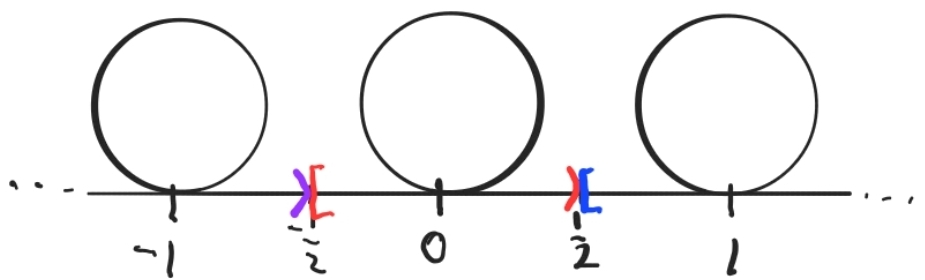
\includegraphics[width=0.7\textwidth]{covering-circles}
\end{proof}

\begin{ex}
	Let $B = \mathbb{S}^2 \cup \lbrace (x, 0, 0) : -1 \leq x \leq 1 \rbrace$.
	Find a simply-connected space $E$ and describe a covering map $p: E \to B$.
\end{ex}
\begin{proof}
	We use the following covering space resembling a necklace of beads:
	\\
	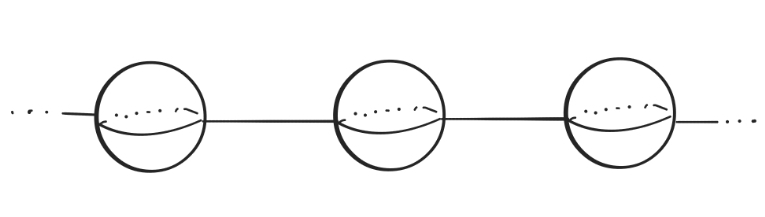
\includegraphics[width=0.7\textwidth]{necklace}
	\\
	We map each $S^2$ to $S^2$ ``identically'' by ``translation'', i.e. we don't do anything special to the points on the spheres.
	Each line segment, modeled from left to right as $[-1, 1]$, is mapped in reverse order: $t \mapsto (-t, 0, 0)$.
	This way, the neighborhoods of points on a sphere not touching a line map locally homeomorphically to points on the sphere not touching the line in $B$, points ``within'' each line map locally homeomorphically to points ``within'' the line in $B$, and the points where the lines and spheres touch map to the points where the line and sphere touch in $B$ so that the neighborhoods are lines sticking out of discs (from the middle, on one side) as desired.
\end{proof}

\end{document}
